\documentclass[11pt]{beamer}
\usepackage[utf8]{inputenc}
\usepackage[T1]{fontenc}
\usepackage{lmodern}
\usetheme{Singapore}
\begin{document}
	\author{Brandelet A., Ducobu L., \textbf{Gamrath S.}}
	\title{La méthode scientifique comme bouclier}
	%\subtitle{}
	%\logo{}
	%\institute{}
	\date{}
	%\subject{}
	%\setbeamercovered{transparent}
	%\setbeamertemplate{navigation symbols}{}
	\begin{frame}[plain]
	\maketitle
\end{frame}
\section{Exemples où ça marche}
\begin{frame}
\frametitle{Expériences : Utilisation de la méthode scientifique}
\begin{itemize}
	\item Cerf-Volant de Franklin
	\item Expérience de Fizeau
%	\item Effet Einstein - De Haas
	\item Décourverte du BEH
	%\item Observation des ondes gravitationelles
	\item ... 
\end{itemize}
\begin{minipage}[c]{0.31\linewidth}
	\begin{center}
		\includegraphics[width=2.5cm]{Franklin} %\vspace{0.2cm}\\
		\\
	\end{center}
\end{minipage}
%\hspace*{\fill} 
\begin{minipage}[c]{0.33\linewidth}
	\begin{center}
		\includegraphics[width=3cm]{Fizeau}\vspace{0.2cm}
	\end{center}
\end{minipage}
%\hspace*{\fill}
\begin{minipage}[c]{0.32\linewidth}
	\begin{center}
		\includegraphics[width=3.5cm]{Beh} %\vspace{0.4cm}
		\end{center}
\end{minipage}

\pause \textbf{NB :} On peut utiliser la méthode scientifique via des simulations numériques, des modèles théoriques ...
\end{frame}
\section{Exemple ou ça ne marche pas}
\subsection{La mémoire de l'eau}
\begin{frame}
\frametitle{La mémoire de l'eau}
\framesubtitle{Qu'est ce que c'est ?}
Publiée dans Nature en 1988
\pause 
\\$\hookrightarrow$ \textbf{Hypothèse} : L’eau qui a été en contact avec certaines substances conserverait une empreinte de certaines propriétés de celles-ci alors qu'elles ne s’y trouvent plus
\pause 
\end{frame}
\begin{frame}
\frametitle{La mémoire de l'eau}
\framesubtitle{Quelle est la contreverse ?}
\begin{itemize}
	\item Résultats obtenus par Jacques  Benveniste et par quatre autres équipes, dont deux en Israël, une au Canada et une autre en Italie. \pause
	\item Dès le mois suivant, la validité des travaux est remise en doute. Les causes principales sont : 
		\begin{itemize}
			\item Mise en cause du protocole expérimental et des conditions de réalisation de l'expérience
			\item Soupçons de conflits d'intérêts
		\end{itemize}  \pause 
	\item En 1993, une équipe utilise le même protocole expérimental et ne parvient pas à reproduire les résultats. Les résultats obtenus sont même l'exact inverse.
\end{itemize}
\end{frame}
\begin{frame}
\frametitle{La mémoire de l'eau}
\framesubtitle{Bizareries}
\begin{itemize}
	\item Le protocole expérimental est remis en cause pour un risque de trop grande influence de l'expérimentateur (comptage des \textit{faux positifs}) \pause 
	\item En 2001, Madeleine Ennis reproduit les résultats de Benveniste en laboratoire en élaborant un protocole étant censé éliminer l'influence de l'expérimentateur. \pause 
	\item Ennis et Benveniste n'arrivent pas à reproduire leurs résultats devant les caméras de la BBC
	\item Bernard Poitevin confirme les résultats de Benveniste en 2008... \pause  Mais était co-auteur de toutes les publications de Benveniste ...
\end{itemize}
\end{frame}
\begin{frame}
\frametitle{La mémoire de l'eau}
\framesubtitle{Bizareries}
\begin{itemize}
	\item Les recherches de Benveniste ont été financées par les laboratoires Boiron, spécialisés dans la vente de produits homéopathiques. 
	\item Beaucoup d'expériences ont tentés de reproduire ces expériences et les résultats sont pour le moins ... mitigés
	\item  La plupart des équipes reproduisant les résultats sont de près ou de loin des collaborateurs de Benveniste
\end{itemize}
\end{frame}
\begin{frame}
\frametitle{La mémoire de l'eau}
\framesubtitle{Que penser de tout cela ?}
\begin{itemize}
	\item La théorie de la mémoire de l'eau n'a toujours pas été validée de manière convaincante
	\item Via la méthode scientifique le manque de réelle reproductibilité incite à la méfiance
	\item Les conflits d'intérêt dûs au financement par une entreprise pharmacieutique pour qui les résultats présentent un intérêt incitent aussi à la méfiance
\end{itemize}
\pause $\hookrightarrow$ Même si on ne sait officiellement pas, l'utilisation de la méthode scientifique incite à la méfiance
\end{frame}
\begin{frame}
\frametitle{La mémoire de l'eau}
\framesubtitle{Et si c'était vrai ?}
Une autre hypothèse est que simplement, leur protocole expérimental est si complexe qu'aucun autre groupe n'est capable de le reproduire et qu'ils ont gardé la recette de leur superbe découverte pour eux.

\end{frame}
\begin{frame}
\frametitle{La mémoire de l'eau}
\framesubtitle{Le mot de la fin}
 Nature a publié l’article en le précédant de la mention : 
 \\ \textit{La rédaction a accepté la publication des résultats par ouverture d’esprit, mais les estime douteux.} 
 \\ \pause
 Le directeur de la revue ajoute qu'il aurait accepté de publier ces travaux pour que Benveniste  ne se fasse passer pour un \\ \textit{Galilée moderne, victime d’une nouvelle Inquisition}
\end{frame}
\subsection{Le monstre du Loch Ness}
\begin{frame}
\frametitle{Le Monstre du Loch Ness}
\framesubtitle{Son observation : Une expérience reproductible ?}
\begin{center}
	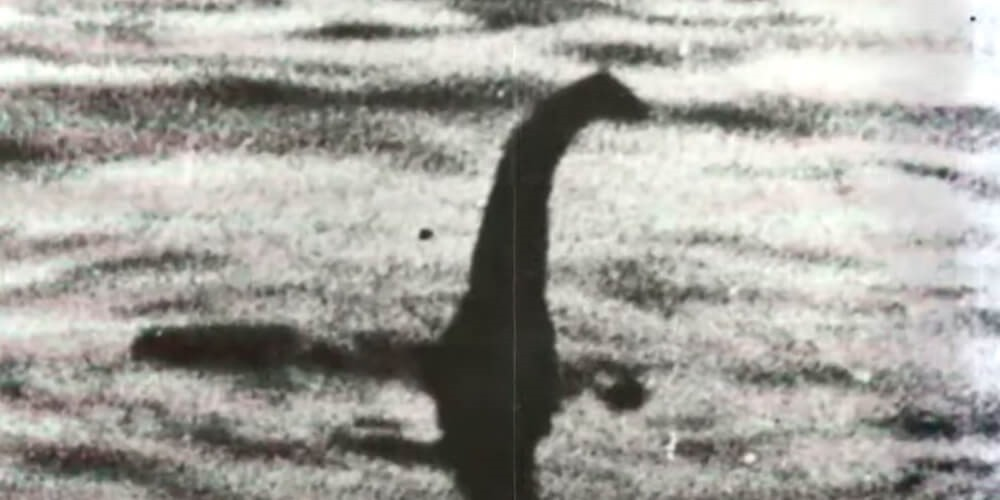
\includegraphics[scale=0.15]{lochness}
\end{center}
\textbf{Liste des observations avec une \textit{preuve}} : 1898, 1935, 1936, 1938 (2x), 1939, 1960, 1962, 1963(2x), 1964, 1965, 1966, 1967(7x), 1968, 1969 (3x), 1975, 1977, 1982, 1985, 2007, 2010, 2015,...
\end{frame}
\begin{frame}
\frametitle{Le Monstre du Loch Ness}
\framesubtitle{Expériences pour montrer son existence}
\textbf{Expériences scientifiques tentant de montrer son existence} : 
\begin{itemize}
	\item 1934 $\rightarrow$ Ce qu'on pensait être le monstre était en fait un phoque
	\item 1968,1969,1970 : Expéditions Sonar (Université de Birmingham) dans le loch $\rightarrow$ Mesures de \textit{grosses masses en mouvement}
	\item 1972,1975,2001 : Expéditions Sonar (Université de Boston) dans le loch $\rightarrow$ RAS $\Rightarrow$ Le monstre est mort
	\item 1987 : Expédition RADAR et Sonar $\rightarrow$ RAS
	\item 2003 : Sondage intensif du loch  $\rightarrow$ RAS
	\item 2018 : Analyse ADN des eaux du Loch. Si monstre il y a, ce ne serait qu'au pire une grosse anguille ...
\end{itemize}
\end{frame}
\begin{frame}
	\frametitle{Le Monstre du Loch Ness}
	\framesubtitle{Identités proposée}
	\begin{itemize}
		\item Un plésiosaure
		\item Une nouvelle espèce de pinnipède
		\item Esturgeon Baltique
		\item Requin du Groenland
		\item Triton géant à long cou
		\item Silure glane
		\item ...
	\end{itemize}
\begin{minipage}[c]{0.31\linewidth}
	\begin{center}
		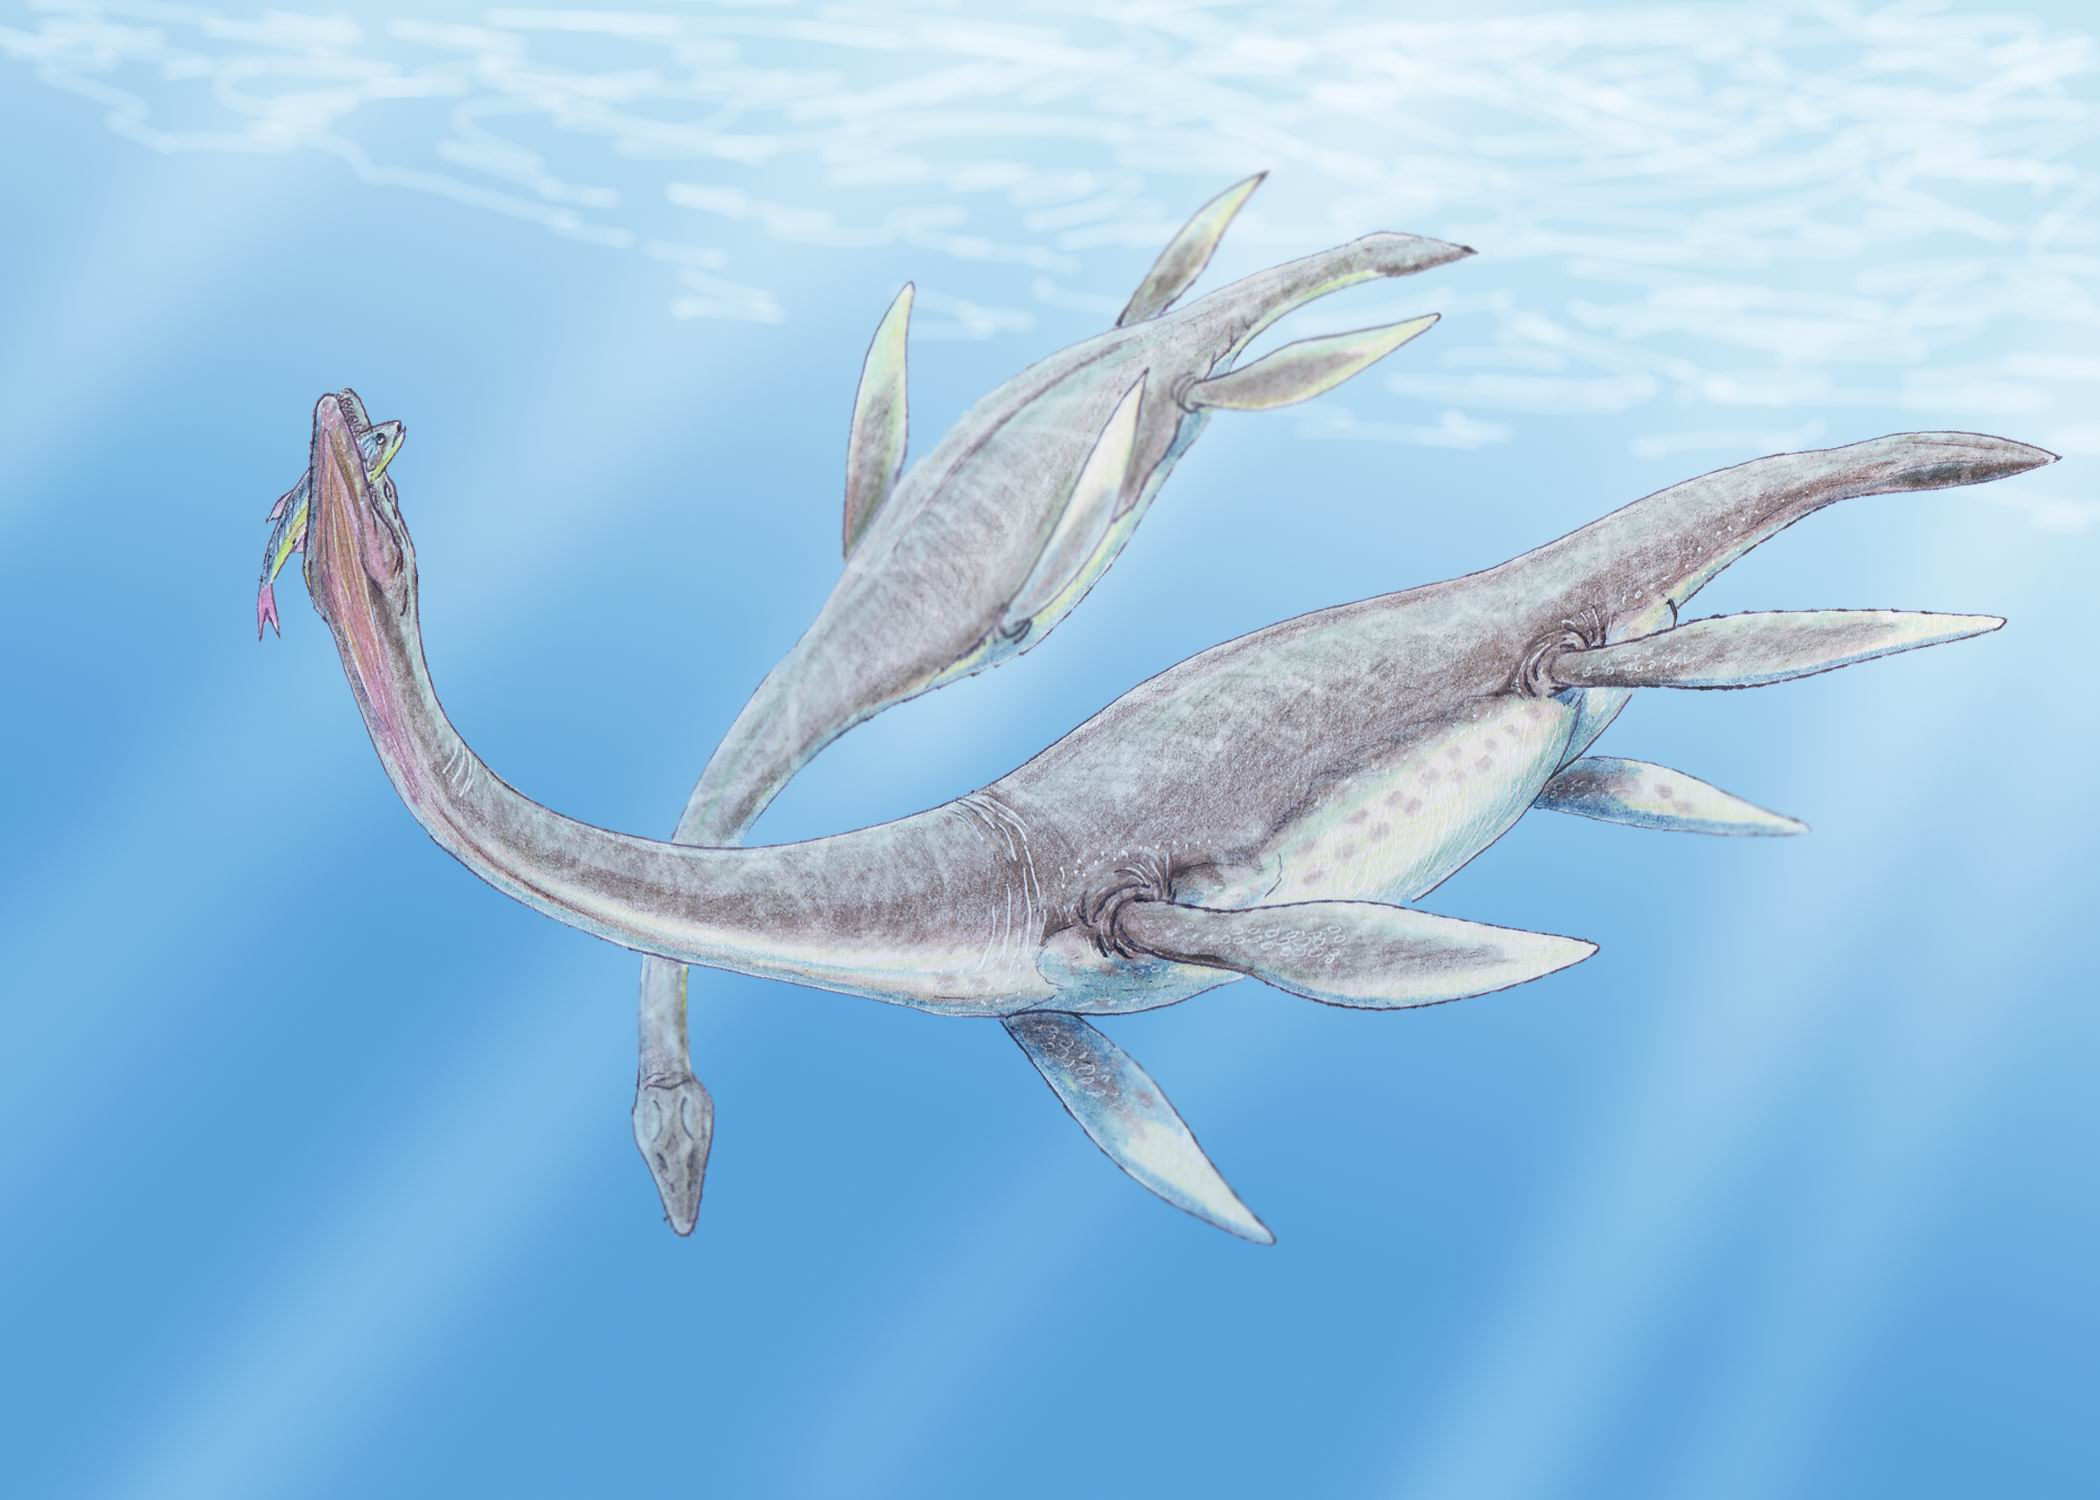
\includegraphics[width=2.5cm]{Plesiosaurus} %\vspace{0.2cm}\\
		\\
	\end{center}
\end{minipage}
%\hspace*{\fill} 
\begin{minipage}[c]{0.33\linewidth}
	\begin{center}
		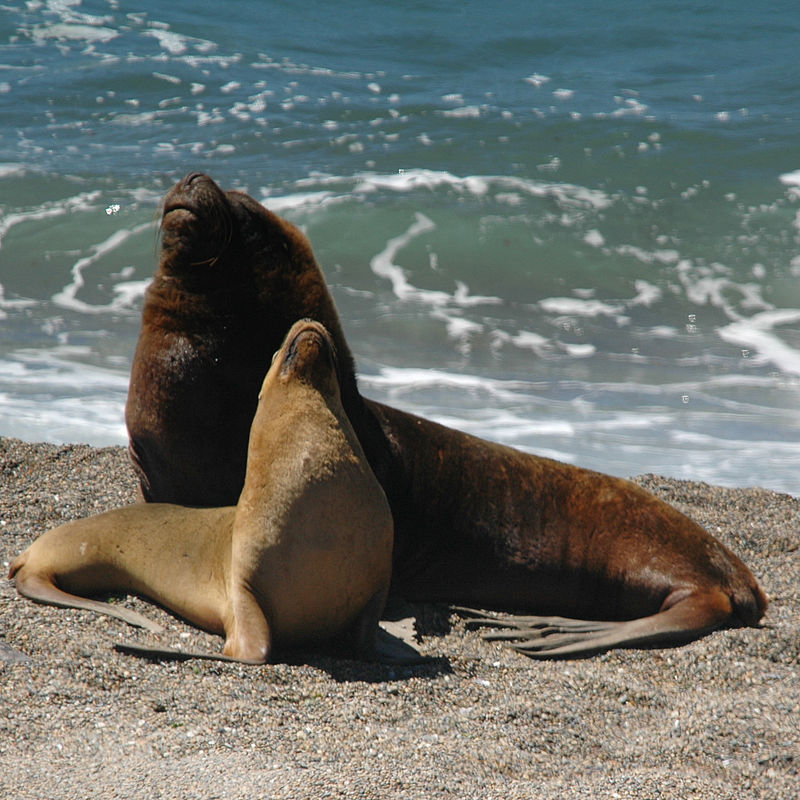
\includegraphics[width=3cm]{pinnipede}\vspace{0.2cm}
	\end{center}
\end{minipage}
%\hspace*{\fill}
\begin{minipage}[c]{0.32\linewidth}
	\begin{center}
		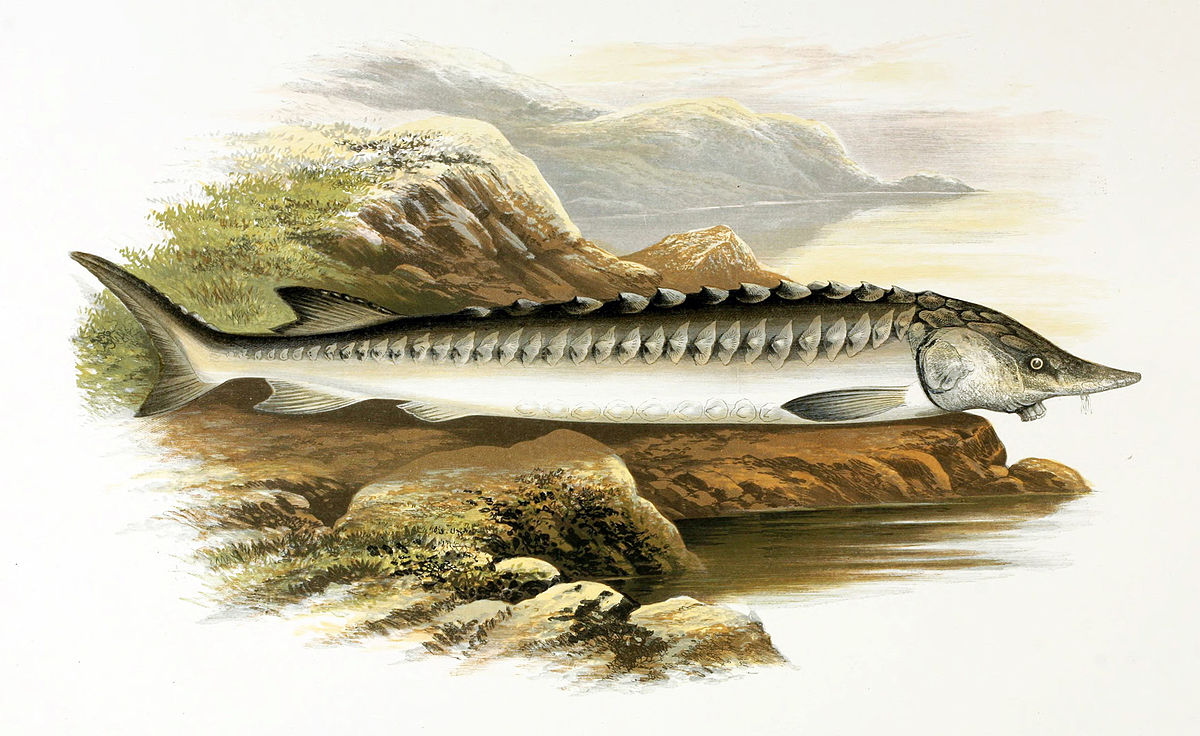
\includegraphics[width=3.5cm]{esturgeon} %\vspace{0.4cm}
	\end{center}
\end{minipage}
\end{frame}
\begin{frame}
\frametitle{Le Monstre du Loch Ness}
\framesubtitle{Canulars avérés - Le mot de la fin}
Un des riverains du Loch Ness aurait déclaré dans son testament qu'il avait sculpté un monstre en bois, et qu'il s'amusait à le sortir pour gonfler la légende.

\pause  On a retrouvé, dans son garage, le modèle en bois du monstre du Loch Ness.
\end{frame}
\end{document}